
\documentclass[fleqn,a4paper,12pt]{article}

% fleqn to left align equations
%\setlength{\textwidth}{2in}
\usepackage{hyperref}
\usepackage{fancyhdr}
\usepackage{enumitem}
%\renewcommand{\familydefault}{\rmdefault}
\renewcommand{\familydefault}{\sfdefault}
%\usepackage{helvet}
%\pagestyle{fancy}
\date{}
%\pagenumbering{gobble}
\usepackage{geometry}
\pagenumbering{gobble}
\usepackage{multicol}
\usepackage{tikz}
\usepackage{amsmath}
\usepackage{amsfonts}
\usepackage{mathtools,xparse}
\usepackage{listings}


%\fancyhf{}
%\pagestyle{fancy}
%\rhead{Mina Jafari}
%\lhead{ML-HW1}
\newcommand{\norm}[1]{\left\lVert#1\right\rVert}

%Abernethy
\newcounter{probnum}
\newcounter{subprobnum}
\newcounter{subsubprobnum}
\stepcounter{probnum}
\stepcounter{subprobnum}
\stepcounter{subsubprobnum}

\newcommand{\nsubprob}[2]{\addtolength{\leftskip}{-3em}\vspace{0em} \noindent \textbf{ \noindent #1) \stepcounter{subprobnum}} #2\par \addtolength{\leftskip}{3em}}

\def \probmargin{1.2em}
\def \probvspace{0em}

\newcommand{\nprob}[2]
{
	
	\vspace{\probvspace}
	\setcounter{subprobnum}{1}
	\setlength{\leftskip}{0em}
	\noindent \arabic{probnum}) \textbf{#1. } #2 
	\vspace{\probvspace}
	\stepcounter{probnum}
}

\newcommand{\subprob}[1]
{
	
	\setlength{\leftskip}{\probmargin}
	\setcounter{subsubprobnum}{1}
	
	\def \subttl{\textbf{(\alph{subprobnum}) }}
	\settowidth{\parindent}{\subttl}
	\addtolength{\leftskip}{\parindent}
	\setlength{\parindent}{-\parindent}
	\subttl #1
	\stepcounter{subprobnum}
	\vspace{\probvspace}
	\setlength{\parindent}{0em}
	
}

\newcommand{\subsubprob}[1]
{
	
	\setlength{\leftskip}{\probmargin}
	\addtolength{\leftskip}{\probmargin}
	
	\def \subttl{\textbf{(\roman{subsubprobnum}) }}
	\settowidth{\parindent}{\subttl}
	\addtolength{\leftskip}{\parindent}
	\setlength{\parindent}{-\parindent}
	\subttl #1
	\stepcounter{subsubprobnum}
	\vspace{\probvspace}
	\setlength{\parindent}{0em}
	
}
%end-abernethy

\geometry{a4paper,left=20mm,right=20mm,top=20mm,bottom=20mm}
%\renewcommand{\headrulewidth}{1.5 pt}

\hypersetup
{
    pdfauthor={Mina Jafari},
    pdfsubject={Homework2},
    pdftitle={MachineLearning},
    pdfkeywords={ML-HW2}
}
\linespread{1.0}

\makeatletter
\newcommand{\hwclass}[1]{\def \TVclass{#1}}
\newcommand{\hwdue}[1]{\def \TVdue{#1}}
\newcommand{\hwassignment}[1]{\def \TVassignment{#1}}
\makeatother

% Title Heading
\renewcommand{\maketitle}
{
	\begin{center}
		\newlength{\titlerulewidth}
		\def \hmwkttl{{\TVclass\, - \TVassignment}}
		\settowidth{\titlerulewidth}{\hmwkttl}
		
		\rule{\titlerulewidth}{1pt}\\[3mm]
		\hmwkttl \\[3mm]
	%	\makebox[\titlerulewidth]{\small \TVname \hspace{1em} \hfill \hfill  group member: Joshua Kammeraad} \\
		\makebox[\titlerulewidth]{\small \TVname \hspace{1em}} \\
		\makebox[\titlerulewidth]{\footnotesize {group member: Joshua Kammeraad} \hspace{1em}} \\
		\rule{\titlerulewidth}{1pt}\\[3mm]
	\end{center}
	
	\vspace{3em}
}

\def\TVname{Mina Jafari}

\hwclass{EECS 545 -- Machine Learning}
\hwdue{11:00pm 01/25/2016}
\hwassignment{Homework \#3}
\begin{document}
\maketitle	

\nprob{Question 1}{
	

\subprob{}{
	\begin{flalign*}
		& t^{(i)} ( {\bf w}^T {\bf x}^{(i)} + b ) \ge 1 - \xi_i\\
		& 1 - t^{(i)} ( {\bf w}^T {\bf x}^{(i)} + b ) \le \xi_i \text{ and } \xi_i \ge 0 \implies\\
		& \xi_i = \max\left(0, 1 - t^{(i)} ( {\bf w}^T {\bf x}^{(i)} + b ) \right)\\
		& \min_{{\bf w}, b}  \frac{1}{2} \Vert{\bf w}\Vert^2 + C \sum_{i=1}^N \xi_i \text{ , substitute for } \xi_i\\
		& \min_{{\bf w}, b}  \frac{1}{2} \Vert{\bf w}\Vert^2 + C \sum_{i=1}^N \max\left(0, 1 - t^{(i)} ( {\bf w}^T {\bf x}^{(i)} + b ) \right) \implies (1) \equiv (2)
	\end{flalign*}
}
	
\subprob{}{
	\begin{flalign*}
		&\text{if } \xi_i^* > 0 \implies \xi_i^* = 1 - t^{(i)} ( {\bf w^*}^T {\bf x}^{(i)} + b^* ) \rightarrow {\bf w^*}^T {\bf x}^{(i)} = \frac{- \xi_i^* + 1}{t^{(i)}} - b^*\\
		&\text{plane: } t^{(i)}((\mathbf{w}^*)^T\mathbf{x}+b^*)-1=0 \rightarrow \mathbf{w^*}^T\mathbf{x} = \frac{1}{t^{(i)}} - b^*\\
		& D=\frac{\Vert({\bf x}^{(i)} - {\bf x}) \cdot {\bf w^*}\Vert}{\Vert{\bf w^*}\Vert} = \frac{\mid ({\bf x}^{(i)})^{\top}{\bf w^*} - {\bf x}^{\top}{\bf w^*} \mid}{\Vert{\bf w^*}\Vert} = \frac{\mid {\bf w^*}^{\top}{\bf x}^{(i)} - {\bf w^*}^{\top}{\bf x} \mid}{\Vert{\bf w^*}\Vert} = \frac{\mid \frac{- \xi_i^* + 1}{t^{(i)}} - b^* - \frac{1}{t^{(i)}} - b^* \mid}{\Vert{\bf w^*}\Vert}\\
		& D=\mid \frac{-\xi_i}{t^{(i)}\Vert{\bf w^*}\Vert}\mid
	\end{flalign*}
		}
		
\subprob{}{
	\begin{flalign*}
		\nabla_{\bf w} E({\bf w}, b) &= \nabla_{\bf w} \frac{1}{2} \Vert{\bf w}\Vert^2 + \nabla_{\bf w} C \sum_{i=1}^N \max\left(0, 1 - t^{(i)} ( {\bf w}^T {\bf x}^{(i)} + b ) \right)\\
		&= {\bf w}+C \sum_{i=1}^N \begin{cases}
		0,& \text{if } t^{(i)} ( {\bf w}^T {\bf x}^{(i)} + b)\geq 1\\
		-t^{(i)}{\bf x}^{(i)}, & \text{if } t^{(i)} ( {\bf w}^T {\bf x}^{(i)} + b) < 1
		\end{cases}\\
		\frac{\partial}{\partial b} E({\bf w}, b) &= \frac{\partial}{\partial b} \frac{1}{2} \Vert{\bf w}\Vert^2 + 	\frac{\partial}{\partial b} C \sum_{i=1}^N \max\left(0, 1 - t^{(i)} ( {\bf w}^T {\bf x}^{(i)} + b ) \right)\\
		&= C \sum_{i=1}^N \begin{cases}
		0,& \text{if } t^{(i)} ( {\bf w}^T {\bf x}^{(i)} + b)\geq 1\\
		-t^{(i)}, & \text{if } t^{(i)} ( {\bf w}^T {\bf x}^{(i)} + b) < 1
		\end{cases}
	\end{flalign*}
}

\subprob{}{
	\begin{figure}[!ht]
		\centering
		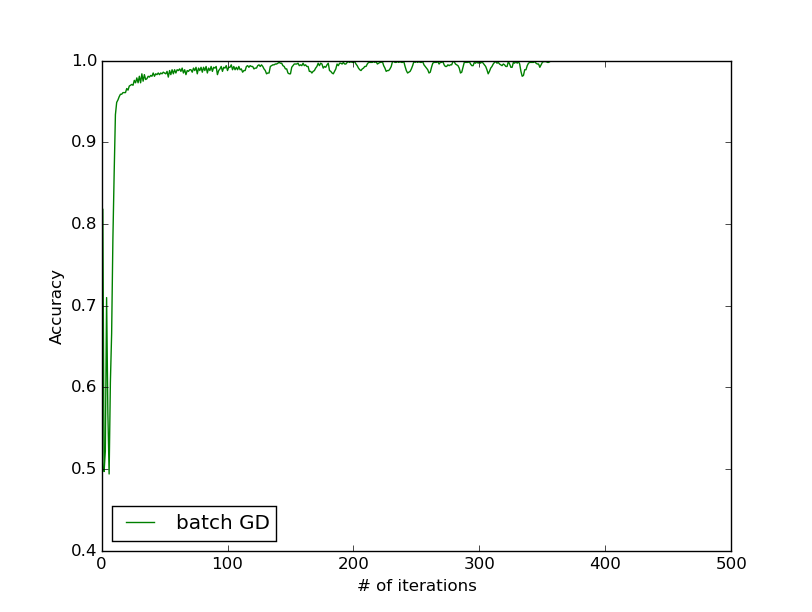
\includegraphics[width=0.5\textwidth]{question-1/1-d.png}
	\end{figure}
	\lstinputlisting[language=Python, basicstyle=\scriptsize]{question-1/q1-d.py}
}

\subprob{}{
	\begin{flalign*}
	\nabla_{\bf w} E^{(i)}({\bf w}, b) &= \nabla_{\bf w} \frac{1}{2N} \Vert{\bf w}\Vert^2 + \nabla_{\bf w} C \max\left(0, 1 - t^{(i)} ( {\bf w}^T {\bf x}^{(i)} + b ) \right)\\
	&= \frac{1}{N}{\bf w}+C \begin{cases}
	0,& \text{if } t^{(i)} ( {\bf w}^T {\bf x}^{(i)} + b)\geq 1\\
	-t^{(i)}{\bf x}^{(i)}, & \text{if } t^{(i)} ( {\bf w}^T {\bf x}^{(i)} + b) < 1
	\end{cases}\\
	\frac{\partial}{\partial b} E^{(i)}({\bf w}, b) &= \frac{\partial}{\partial b} \frac{1}{2N} \Vert{\bf w}\Vert^2 + \frac{\partial}{\partial b} C \max\left(0, 1 - t^{(i)} ( {\bf w}^T {\bf x}^{(i)} + b ) \right)\\
	&= C \begin{cases}
	0,& \text{if } t^{(i)} ( {\bf w}^T {\bf x}^{(i)} + b)\geq 1\\
	-t^{(i)}, & \text{if } t^{(i)} ( {\bf w}^T {\bf x}^{(i)} + b) < 1
	\end{cases}
	\end{flalign*}	
}

\subprob{}{
		\begin{figure}[!ht]
			\centering
			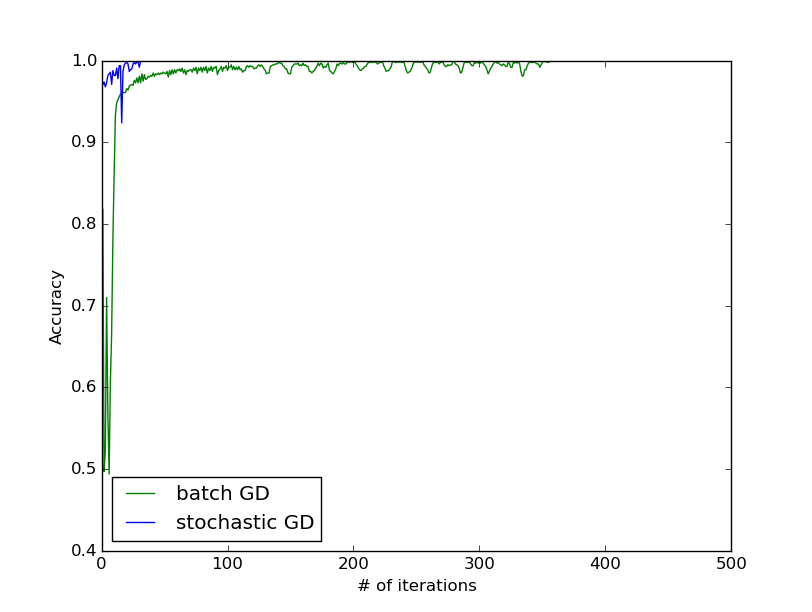
\includegraphics[width=0.5\textwidth]{question-1/1-df.png}
		\end{figure}
		\lstinputlisting[language=Python, basicstyle=\scriptsize]{question-1/q1-f.py}	
}

\subprob{}{
	Stochastic GD converges after about 30 iterations while it takes about 350 steps for the batch GD to converge, so in this case, it's roughly 12 times faster. Based on the plot!
}

\subprob{}{
	\begin{align*}
		& \min_{{\bf w}, b} & & \frac{1}{2} \Vert{\bf w}\Vert^2 + C \sum_{i=1}^N \xi_i \\
		& \text{subject to} & & t^{(i)} ( {\bf w}^T {\bf x}^{(i)} + b ) \ge 1 - \xi_i\\
		& & & \xi_i \ge 0 \qquad (i = 1, \ldots, N)
	\end{align*}
	\begin{flalign*}
		& g_1: \xi_i \ge 0, g_2: t^{(i)} ( {\bf w}^T {\bf x}^{(i)} + b ) - 1 + \xi_i \ge 0\\
		& \mathcal{L}({\bf w}, b, \xi_i, \alpha, \mu)=\frac{1}{2} \Vert{\bf w}\Vert^2 + C \sum_{i=1}^N \xi_i - \sum_{i=1}^N \alpha_i \big(t^{(i)} ( {\bf w}^T {\bf x}^{(i)} + b ) - 1 + \xi_i\big) - \sum_{i=1}^{N} \mu_i \xi_i\\
		& \nabla_{\bf w}\mathcal{L}={\bf w} - \sum_{i=1}^{N} \alpha_i t^{(i)}{\bf x}^{(i)}=0 \rightarrow {\bf w}=\sum_{i=1}^{N}\alpha_i t^{(i)}{\bf x}^{(i)}\\
		& \frac{\partial \mathcal{L}}{\partial b}=-\sum_{i=1}^{N} \alpha_i t^{(i)}=0\\
		& \frac{\partial \mathcal{L}}{\partial \xi_i}=C - \alpha_i - \mu_i =0 \rightarrow \alpha_i=C-\mu_i\\
		& \mathcal{L_D}(\alpha, \mu)=\frac{1}{2}\bigg(\sum_{i=1}^{N}\alpha_i t^{(i)}{\bf x}^{(i)}\bigg)^2 + C\sum_{i=1}^{N}\xi_i - \sum_{i=1}^{N}\alpha_i \big(t^{(i)} \sum_{j=1}^{N}\alpha_j t^{(j)}{\bf x}^{(j)}{\bf x}^{(i)} + t^{(i)} b -1+\xi_i\big) \\ &- \sum_{i=1}^{N}\mu_i\xi_i\\
		&= \frac{1}{2}\sum_{i=1}^{N}\sum_{j=1}^{N}\alpha_i \alpha_j t^{(i)}t^{(j)}({\bf x}^{(i)})^{\top}{\bf x}^{(j)} + C\sum_{i=1}^{N}\xi_i - \sum_{i=1}^{N}\sum_{j=1}^{N}\alpha_i \alpha_j t^{(i)}t^{(j)}({\bf x}^{(i)})^{\top}{\bf x}^{(j)}\\ &- \sum_{i=1}^{N} \alpha_i t^{(i)} b - \sum_{i=1}^{N}\alpha_i - \sum_{i=1}^{N} \alpha_i\xi_i - \sum_{i=1}^{N}\mu_i\xi_i\\
		& \text{substitute } \alpha_i \text{ by } C-\mu_i \text{ in second to the last term} \implies\\
		&=\frac{1}{2}\sum_{i=1}^{N}\sum_{j=1}^{N}\alpha_i \alpha_j t^{(i)}t^{(j)}({\bf x}^{(i)})^{\top}{\bf x}^{(j)} - \sum_{i=1}^{N}\sum_{j=1}^{N}\alpha_i \alpha_j t^{(i)}t^{(j)}({\bf x}^{(i)})^{\top}{\bf x}^{(j)} - b \sum_{i=1}^{N} \alpha_i t^{(i)} - \sum_{i=1}^{N}\alpha_i \\
		&\mathcal{L_D}(\alpha, \mu)=-\frac{1}{2}\sum_{i=1}^{N}\sum_{j=1}^{N}\alpha_i \alpha_j t^{(i)}t^{(j)}({\bf x}^{(i)})^{\top}{\bf x}^{(j)} - \sum_{i=1}^{N}\alpha_i \\
		& k({\bf x}_i, {\bf x}_j)=({\bf x}^{(i)})^{\top}{\bf x}^{(j)} \implies \mathcal{L_D}(\alpha, \mu)=-\frac{1}{2}\sum_{i=1}^{N}\sum_{j=1}^{N}\alpha_i \alpha_j t^{(i)}t^{(j)}k({\bf x}_i, {\bf x}_j) - \sum_{i=1}^{N}\alpha_i
	\end{flalign*}
	
}

\subprob{}{
	Training accuracy: 99.9\% \\
	Test accuracy: 98\% \\
	Parameters: C=1.0, gamma=$5 \times 10^{-7}$, tol=0.0001 \\
	\begin{figure}[htp]
		\centering
		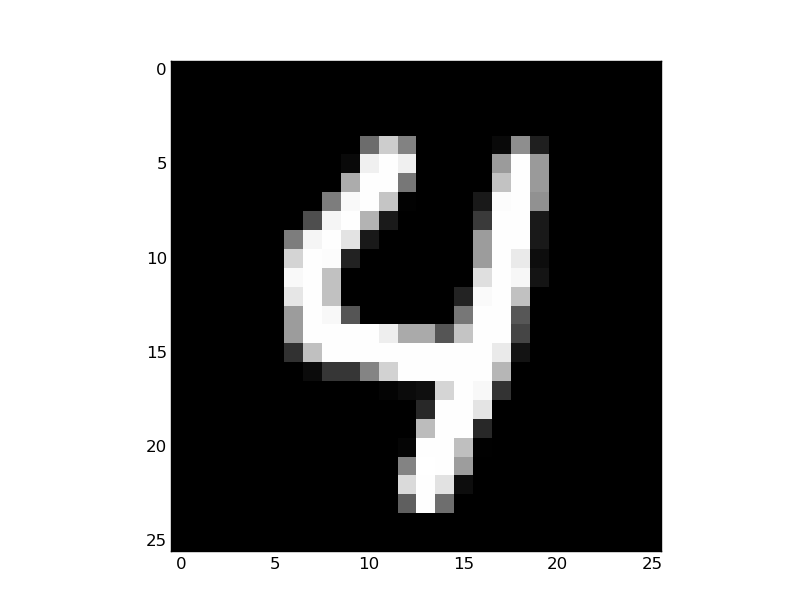
\includegraphics[width=.2\textwidth]{question-1/1-i-1.png}\quad
		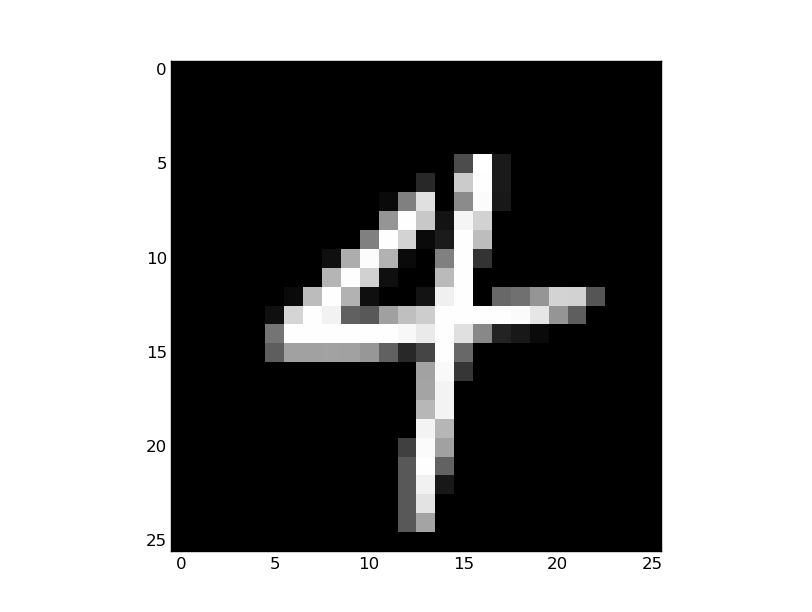
\includegraphics[width=.2\textwidth]{question-1/1-i-2.png}\quad
		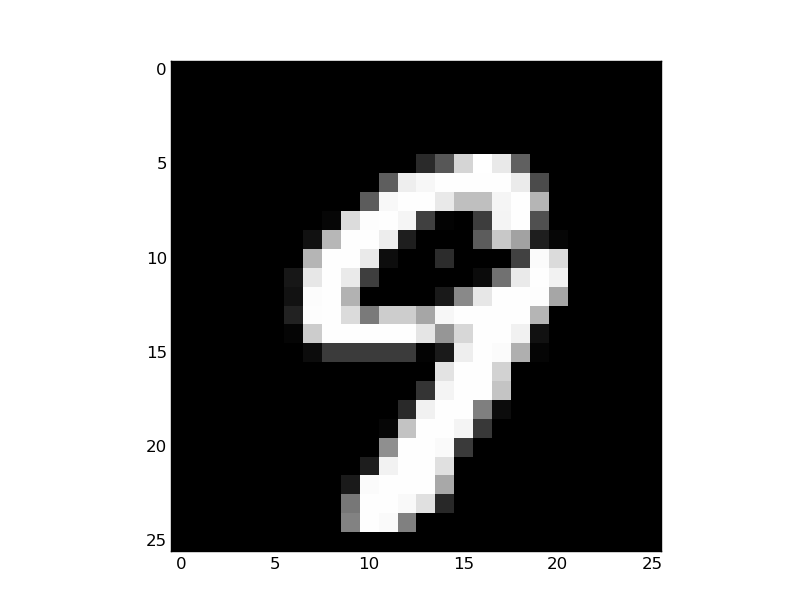
\includegraphics[width=.2\textwidth]{question-1/1-i-3.png}
		
		\medskip
		
		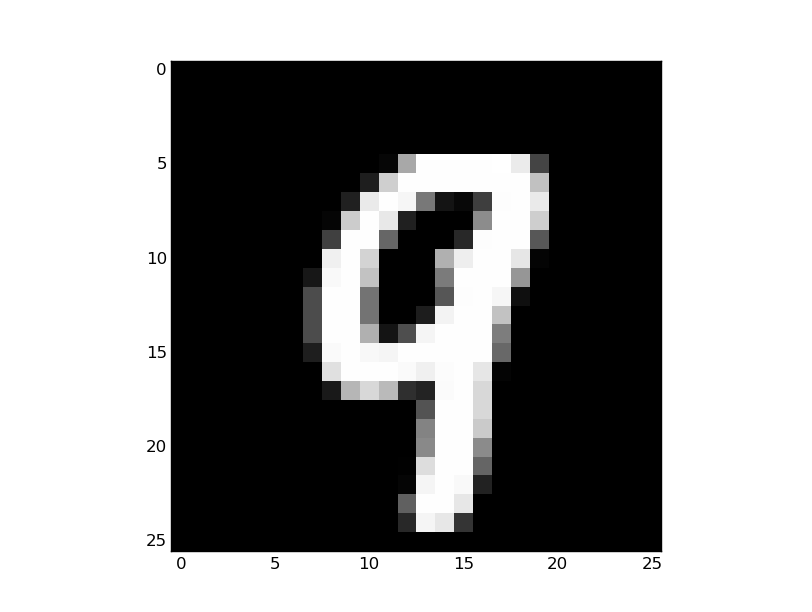
\includegraphics[width=.2\textwidth]{question-1/1-i-4.png}\quad
		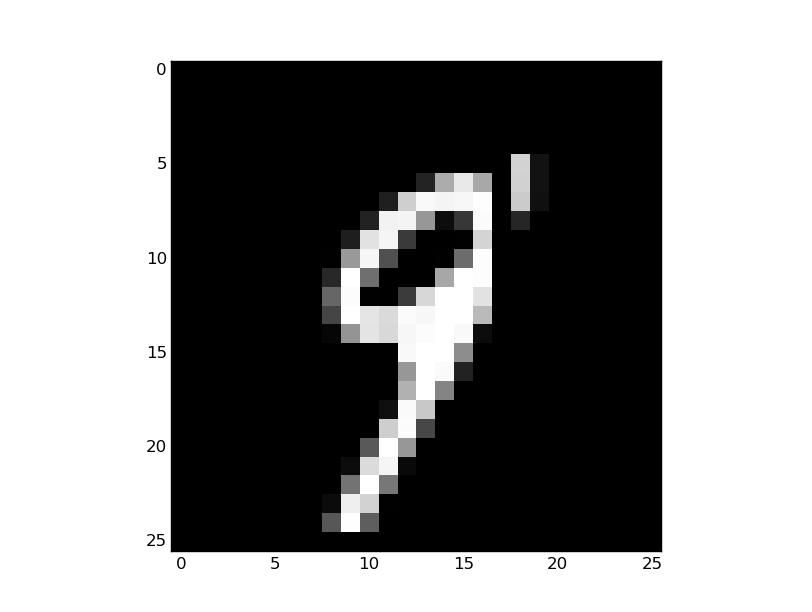
\includegraphics[width=.2\textwidth]{question-1/1-i-5.png}
	\end{figure}
	\lstinputlisting[language=Python, basicstyle=\scriptsize]{question-1/q1-i.py}
}

\subprob{
	}
}

\vspace{20cm}

\nprob{Question 2}{
	\lstinputlisting[language=Python, basicstyle=\scriptsize]{question-2/q2.py}
	 }

\vspace{30cm}
\nprob{Question 3}{
	\subprob{}{
		\begin{flalign*}
		k(\mathbf{u}, \mathbf{v}) &=(\langle \mathbf{u}, \mathbf{v}\rangle+1)^4 \\
		&=(\mathbf{u}^{\top} \mathbf{v}+1)^4 \\
		&=(\mathbf{u}^{\top} \mathbf{v})^4+4(\mathbf{u}^{\top} \mathbf{v})^3+6(\mathbf{u}^{\top} \mathbf{v})^2+4(\mathbf{u}^{\top} \mathbf{v})+1 \\
		&=\big(\sum_{i=1}^{d} \mathbf{u}_i \mathbf{v}_i\big)^4+4\big(\sum_{i=1}^{d} \mathbf{u}_i \mathbf{v}_i\big)^3+6\big(\sum_{i=1}^{d} \mathbf{u}_i \mathbf{v}_i\big)^2+4\big(\sum_{i=1}^{d} \mathbf{u}_i \mathbf{v}_i\big)+1 \\
		&=\sum_{k_1+...+k_m=4}\dbinom{4}{k_1,...,k_m}\prod_{1\leq t\leq m}(\mathbf{u}_t \mathbf{v}_t)^{k_t} + 4 \sum_{k_1+...+k_m=3}\dbinom{3}{k_1,...,k_m}\prod_{1\leq t\leq m}(\mathbf{u}_t \mathbf{v}_t)^{k_t}\\ 
		&+6 \sum_{k_1+...+k_m=2}\dbinom{2}{k_1,...,k_m}\prod_{1\leq t\leq m}(\mathbf{u}_t \mathbf{v}_t)^{k_t} + 4\big(\sum_{i=1}^{d} \mathbf{u}_i \mathbf{v}_i\big)  + 1\\
		&=\phi(\mathbf{u})^\top \phi(\mathbf{v})\\
		&\implies \phi (\mathbf{x}) = \sqrt{\sum_{k_1+...+k_m=4}\dbinom{4}{k_1,...,k_m}}\prod_{1\leq t\leq m}(\mathbf{x}_t)^{k_t} \\
		&+\sqrt{4 \sum_{k_1+...+k_m=3}\dbinom{3}{k_1,...,k_m}}\prod_{1\leq t\leq m}(\mathbf{x}_t)^{k_t}+\sqrt{6 \sum_{k_1+...+k_m=2}\dbinom{2}{k_1,...,k_m}}\prod_{1\leq t\leq m}(\mathbf{x}_t)^{k_t}\\
		&+ 2\big(\sum_{i=1}^{d}\mathbf{x}_i\big) + 1
		\end{flalign*}
	}
	\subprob{}{
		\subsubprob{}{
			PD
			\begin{flalign*}
				k({\bf x}, {\bf z}) &= k_1({\bf x}, {\bf z}) + k_2({\bf x}, {\bf z})\\
									&=\phi_1(\mathbf{x})^{\top}\phi_1(\mathbf{z}) + \phi_2(\mathbf{x})^{\top}\phi_2(\mathbf{z})\\
									&=\sum_{i=1}^{m}\phi_1(\mathbf{x})_i\phi_1(\mathbf{z})_i + \sum_{j=1}^{n}\phi_2(\mathbf{x})_j\phi_2(\mathbf{z})_j\\
									%&=\sum_{i=1}^{m}\phi_1(\mathbf{x}_i)\phi_1(\mathbf{z}_i)\phi_2(\mathbf{x}_i)\phi_2(\mathbf{z}_i)\\
									%&=\sum_{i=1}^{m}\phi_1(\mathbf{x}_i)\phi_2(\mathbf{x}_i)\phi_1(\mathbf{z}_i)\phi_2(\mathbf{z}_i)\\
									%&=\phi_1(\mathbf{x})^{\top}\phi_2(\mathbf{x})^{\top}\phi_1(\mathbf{z})\phi_2(\mathbf{z})\\
									&=\sum_{i=1}^{m}\phi_1(\mathbf{x}_1)_i\phi_1(\mathbf{z}_1)_i + \dotsc + \sum_{i=1}^{m}\phi_1(\mathbf{x}_D)_i\phi_1(\mathbf{z}_D)_i\\
									&+\sum_{j=1}^{n}\phi_2(\mathbf{x}_1)_j\phi_2(\mathbf{z}_1)_j + \dotsc + \sum_{j=1}^{n}\phi_2(\mathbf{x}_D)_j\phi_2(\mathbf{z}_D)_j\\
									& \implies \phi(\mathbf{y}) = \{\phi_1(\mathbf{y}), \phi_2(\mathbf{y})\}
			\end{flalign*}			
			}
		\subsubprob{}{
			Not PD
			\begin{flalign*}
			k({\bf x}, {\bf z}) &= k_1({\bf x}, {\bf z}) - k_2({\bf x}, {\bf z})\\
								&= {\bf x}^{\top}{\bf z} - ({\bf x}^{\top}{\bf z})^2\\
								&=2 \times 1 - (2 \times 1)^2 = -2
			\end{flalign*}
		}
		\subsubprob{}{
			PD
			\begin{flalign*}
				k({\bf x}, {\bf z}) &= a k_1({\bf x}, {\bf z})\\
									&= a \phi_1(\mathbf{x})^{\top}\phi_1(\mathbf{z})\\
									&= a \sum_{i=1}^{m}\phi_1(\mathbf{x})_i\phi_1(\mathbf{z})_i\\
									&= \sum_{i=1}^{m}\sqrt{a}\phi_1(\mathbf{x})_i\sqrt{a}\phi_1(\mathbf{z})_i\\
									&= \big( \sqrt{a}\phi_1(\mathbf{x}) \big)^{\top} \big( \sqrt{a}\phi_1(\mathbf{z}) \big)\\
									&\implies \phi(\mathbf{y}) = \sqrt{a}\phi_1(\mathbf{y})
			\end{flalign*}
		}
		\subsubprob{}{
			PD
			\begin{flalign*}
				k({\bf x}, {\bf z}) &= k_1({\bf x}, {\bf z}) k_2({\bf x}, {\bf z})\\
									&=\phi_1(\mathbf{x})^{\top}\phi_1(\mathbf{z})\phi_2(\mathbf{x})^{\top}\phi_2(\mathbf{z})\\
									&=\sum_{i=1}^{m}\phi_1(\mathbf{x})_i\phi_1(\mathbf{z})_i  \sum_{j=1}^{n}\phi_2(\mathbf{x})_j\phi_2(\mathbf{z})_j\\
									&=\sum_{i=1}^{m}\sum_{j=1}^{n}\phi_1(\mathbf{x})_i\phi_1(\mathbf{z})_i\phi_2(\mathbf{x})_j\phi_2(\mathbf{z})_j\\
									&\implies \phi(\mathbf{y}) = \phi_1(\mathbf{y})\phi_2(\mathbf{y})
			\end{flalign*}
		}
		\subsubprob{}{
			PD
			\begin{flalign*}
				k({\bf x}, {\bf z}) &= f({\bf x}) f({\bf z}) = \phi(\mathbf{x})^{\top} \phi(\mathbf{z}) \\
				&\text{the output of } f(\mathbf{y})\text{ is a scalar} \implies f(\mathbf{y})f(\mathbf{y}) \text{ is an inner product} \\
				\phi(\mathbf{y}) &= f(\mathbf{y})
			\end{flalign*}
		}
		\subsubprob{}{
			PD
			\begin{flalign*}
				k({\bf x}, {\bf z}) &= c_0 + c_1 k_1({\bf x}, {\bf z}) + c_2 (k_1({\bf x}, {\bf z}))^2 + \cdots + c_n (k_1({\bf x}, {\bf z}))^n\\
									& k_1({\bf x}, {\bf z}) = \phi({\bf x})^{\top} \phi({\bf z})\\
				k({\bf x}, {\bf z}) &= c_0 + c_1 \phi({\bf x})^{\top} \phi({\bf z}) + c_2 (\phi({\bf x})^{\top} \phi({\bf z}))^2 + \cdots + c_n (\phi({\bf x})^{\top} \phi({\bf z}))^n\\
									&= c_0 + \sqrt{c_1} \phi({\bf x})^{\top} \sqrt{c_1}\phi({\bf z}) + \sqrt{c_2} (\phi({\bf x})^{\top})^2 \sqrt{c_2}(\phi({\bf z}))^2 + \cdots + \sqrt{c_n} (\phi({\bf x})^{\top})^n \sqrt{c_n}(\phi({\bf z}))^n\\
									&\implies \phi({\bf y}) = \{ \sqrt{c_0}, \sqrt{c_1} \phi({\bf y}), \sqrt{c_2} (\phi({\bf y}))^2, \cdots , \sqrt{c_n} (\phi({\bf x}))^n \}
			\end{flalign*}
		}
		\subsubprob{}{
			\begin{flalign*}
				e^x &= \sum_{n=0}^{\infty} \frac{x^n}{n!} = 1 + x + \frac{x^2}{2!} + \frac{x^3}{3!} + \dots \\
				k({\bf x}, {\bf z}) &= \exp\left(\frac{-\Vert{\bf x}-{\bf z}\Vert^2}{2\sigma^2}\right) = \exp\left(\frac{-({\bf x}-{\bf z})({\bf x}-{\bf z})}{2\sigma^2}\right)\\
									&= \exp\left(\frac{-{\bf x}^2}{2\sigma^2}\right)\exp\left(\frac{-{\bf z}^2}{2\sigma^2}\right)\exp\left(\frac{2{\bf xz}}{2\sigma^2}\right)\\
									%&= \sum_{n=0}^{\infty}\frac{1}{n!}\bigg(\frac{-{\bf x}^2}{2\sigma^2} \bigg)^n \sum_{m=0}^{\infty}\frac{1}{m!}\bigg(\frac{-{\bf z}^2}{2\sigma^2} \bigg)^m \sum_{k=0}^{\infty}\frac{1}{k!}\bigg(\frac{2{\bf xz}^2}{2\sigma^2} \bigg)^k\\
									&= \sum_{n=0}^{\infty}\frac{1}{n!}\bigg(\frac{-{\bf x}^2}{2\sigma^2} \bigg)^n \sum_{n=0}^{\infty}\frac{1}{n!}\bigg(\frac{-{\bf z}^2}{2\sigma^2} \bigg)^n \sum_{n=0}^{\infty}\frac{1}{n!}\bigg(\frac{{\bf xz}}{\sigma^2} \bigg)^n\\
									%&= \frac{1}{n!m!k!}\sum_{n=0}^{\infty}\sum_{m=0}^{\infty}\sum_{k=0}^{\infty}\bigg(\frac{-{\bf x}^2}{2\sigma^2} \bigg)^n \bigg(\frac{-{\bf z}^2}{2\sigma^2} \bigg)^m \bigg(\frac{2{\bf xz}}{2\sigma^2} \bigg)^k\\
									%&= \frac{1}{n!m!k!}\sum_{n=0}^{\infty}\sum_{m=0}^{\infty}\sum_{k=0}^{\infty}\bigg(\frac{-{\bf x}^2}{2\sigma^2} \bigg)^n \bigg(\frac{-{\bf z}^2}{2\sigma^2} \bigg)^m \bigg(\frac{{\bf x}}{\sigma} \bigg)^k \bigg(\frac{{\bf z}}{\sigma} \bigg)^k\\
									&= \sum_{n=0}^{\infty}\frac{1}{n!}\bigg(\frac{-{\bf x}^2}{2\sigma^2} \bigg)^n \sum_{n=0}^{\infty}\frac{1}{n!}\bigg(\frac{-{\bf z}^2}{2\sigma^2} \bigg)^n \sum_{n=0}^{\infty}\frac{1}{n!}\bigg(\frac{{\bf x}}{\sigma} \bigg)^n \bigg(\frac{{\bf z}}{\sigma} \bigg)^n\\
									& \implies \phi(\mathbf{y}) = \sum_{n=0}^{\infty}\frac{1}{n!}\bigg(\frac{-{\bf y}^2}{2\sigma^2} \bigg)^n \sum_{n=0}^{\infty}\sqrt{\frac{1}{n!}} \bigg(\frac{{\bf y}}{\sigma} \bigg)^n
				%k({\bf x}, {\bf z}) &= \exp\left(\frac{-\Vert{\bf x}-{\bf z}\Vert^2}{2\sigma^2}\right) = \sum_{n=0}^{\infty}\frac{1}{n!}\bigg(\frac{-\Vert{\bf x}-{\bf 				
										%z}\Vert^2}{2\sigma^2}\bigg)^n\\ 
									%&= \sum_{n=0}^{\infty}\frac{1}{n!}\bigg(\frac{-\langle \mathbf{x-z},\mathbf{x-z}\rangle}{2\sigma^2}\bigg)^n = \sum_{n=0}^{\infty}\frac{1}{n!}\frac{1}{(-2\sigma^2)^n}\bigg(\langle \mathbf{x-z},\mathbf{x-z}\rangle\bigg)^n \\
									%&= \sum_{n=0}^{\infty}\frac{1}{n!}\frac{1}{(-2\sigma^2)^n}\bigg( \sum_{i=1}^{D} (x_i-z_i)(x_i-z_i) \bigg)^n = \sum_{n=0}^{\infty}\frac{1}{n!}\frac{1}{(-2\sigma^2)^n}\bigg( \sum_{i=1}^{D} (x_i-z_i)^2 \bigg)^n \\
									%&= \sum_{n=0}^{\infty}\frac{1}{n!}\frac{1}{(-2\sigma^2)^n} \sum_{k_1+...+k_D=n}\dbinom{n}{k_1,...,k_D}\prod_{1\leq t\leq D}\big((x_t-z_t)^2\big)^{k_t}\\
									%&= \sum_{n=0}^{\infty}\frac{1}{n!}\frac{1}{(-2\sigma^2)^n} \sum_{k_1+...+k_D=n}\dbinom{n}{k_1,...,k_D}\prod_{1\leq t\leq D}\big((x_t)^2+(z_t)^2-2(x_t)(z_t)\big)^{k_t}\\
									%&= \sum_{n=0}^{\infty}\frac{1}{n!}\frac{1}{(-2\sigma^2)^n} \sum_{k_1+...+k_D=n}\dbinom{n}{k_1,...,k_D}\prod_{1\leq t\leq D}  
									%\bigg( \sum_{j_1+...+j_m=k_t}\dbinom{k_t}{j_1,...,j_m}\prod_{1\leq v\leq m} (a_v)^{k_v} \bigg)\\
									%& a_v \in \{ x_t^2, z_t^2,-2x_t z_t \}\\
									%\phi(\mathbf{y}) &= \sqrt{\sum_{n=0}^{\infty}\frac{1}{n!}\frac{1}{(-2\sigma^2)^n} \sum_{k_1+...+k_D=n}\dbinom{n}{k_1,...,k_D}\prod_{1\leq t\leq D}  
										%\bigg( \sum_{j_1+...+j_m=k_t}\dbinom{k_t}{j_1,...,j_m}\prod_{1\leq v\leq m} ????}
			\end{flalign*}
		}

	}
}

\vspace{30cm}
\nprob{Question 4}{
	\subprob{}{
		\begin{flalign*}
			\hat{f}(\mathbf{x})&=\hat{\mathbf{w}}^T\phi(\mathbf{x})=\mathbf{t}^T\Phi(\Phi^T\Phi + \lambda I)^{-1}\phi(\mathbf{x})\\
			(P+QRS)^{-1}&=P^{-1}-P^{-1}Q(R^{-1}+SP^{-1}Q)^{-1}SP^{-1}, P=\lambda I, Q=\Phi^{\top}, R=I, S=\Phi\\
			\hat{f}(\mathbf{x})
			&=\mathbf{t}^T\Phi\big[\lambda^{-1}I - \lambda^{-1}I \Phi^T(I+\Phi\lambda^{-1}I\Phi^T)^{-1}\Phi\lambda^{-1}I \big]\phi(\mathbf{x})\text{   }, {\bf K}=\Phi\Phi^T, k({\bf x})=\Phi\phi({\bf x})\\
			&=\mathbf{t}^T\big[\Phi\lambda^{-1}I - \Phi\lambda^{-1}I \Phi^T(I+\Phi\lambda^{-1}I\Phi^T)^{-1}\Phi\lambda^{-1}I \big]\phi(\mathbf{x})\\
			&=\mathbf{t}^T\big[\Phi\lambda^{-1}I\phi(\mathbf{x}) - \Phi\lambda^{-1}I \Phi^T(I+\Phi\lambda^{-1}I\Phi^T)^{-1}\Phi\lambda^{-1}I\phi(\mathbf{x}) \big]\\
			&=\mathbf{t}^T\big[\lambda^{-1}Ik({\bf x}) - \lambda^{-1}I {\bf K}(I+\lambda^{-1}I{\bf K})^{-1}\lambda^{-1}Ik({\bf x}) \big]\\
			&=\mathbf{t}^T\big[I - \lambda^{-1}I {\bf K}(I+\lambda^{-1}I{\bf K})^{-1} \big]\big(\lambda^{-1}Ik({\bf x})\big)\\
			&=\mathbf{t}^T\big[I - \lambda^{-1}I {\bf K}(I+\lambda^{-1}I{\bf K})^{-1} \big](I+\lambda^{-1}I{\bf K})(I+\lambda^{-1}I{\bf K})^{-1}\big(\lambda^{-1}Ik({\bf x})\big)\\
			&=\mathbf{t}^T\big[(I+\lambda^{-1}I{\bf K}) - \lambda^{-1}I {\bf K} \big](I+\lambda^{-1}I{\bf K})^{-1}\big(\lambda^{-1}Ik({\bf x})\big)\\
			&=\mathbf{t}^T I(I+\lambda^{-1}I{\bf K})^{-1}\big(\lambda^{-1}Ik({\bf x}) \big)\\
			&=\big[\mathbf{t}^T(\lambda I+{\bf K})^{-1}k({\bf x})\big]^T\\
			&=k({\bf x})(\lambda I+{\bf K})^{-1}\mathbf{t}\\
			\hat{\mathbf{w}}&=(\Phi^T\Phi + \lambda I)^{-1}\Phi^T\mathbf{t}\\
			&=\big[\lambda^{-1}I - \lambda^{-1}I \Phi^T(I+\Phi\lambda^{-1}I\Phi^T)^{-1}\Phi\lambda^{-1}I \big]\Phi^T\mathbf{t}\\
			&=\big[\lambda^{-1}I\Phi^T - \lambda^{-1}I \Phi^T(I+\Phi\lambda^{-1}I\Phi^T)^{-1}\Phi\lambda^{-1}I\Phi^T \big]\mathbf{t}\\
			&=\big[\lambda^{-1}I\Phi^T - \lambda^{-1}I \Phi^T(I+\lambda^{-1}I{\bf K})^{-1}\lambda^{-1}I{\bf K} \big]\mathbf{t}\\
			&=(\lambda^{-1}I\Phi^T)(\lambda I+{\bf K})^{-1}(\lambda I+{\bf K})\big[I - (\lambda I+{\bf K})^{-1}{\bf K} \big]\mathbf{t}\\
			&=(\lambda^{-1}I\Phi^T)(\lambda I+{\bf K})^{-1}\big[(\lambda I+{\bf K}) - {\bf K} \big]\mathbf{t}\\
			&=(\lambda\lambda^{-1}I\Phi^T)(\lambda I+{\bf K})^{-1}\mathbf{t}\\
			&=\Phi^T(\lambda I+{\bf K})^{-1}\mathbf{t}\\
			&=\Phi^T {\bf a}
		\end{flalign*}

	}
	\subprob{}{
		\subsubprob{}
		{
			RMSE = 10.8899710344
			
			\lstinputlisting[language=Python, basicstyle=\scriptsize]{question-4/q4-b-i.py}
			}
		\subsubprob{}
		{
			RMSE = 10.0965667265
			
			\lstinputlisting[language=Python, basicstyle=\scriptsize]{question-4/q4-b-ii.py}
			}
		\subsubprob{}
		{
			RMSE = 9.31271021985
			
			\lstinputlisting[language=Python, basicstyle=\scriptsize]{question-4/q4-b-iii.py}
			}
		\subsubprob{}
		{
			RMSE = 12.0441706978
			
			\lstinputlisting[language=Python, basicstyle=\scriptsize]{question-4/q4-b-vi.py}
			}

		}

}

\end{document}